% This file was created with tikzplotlib v0.10.1.
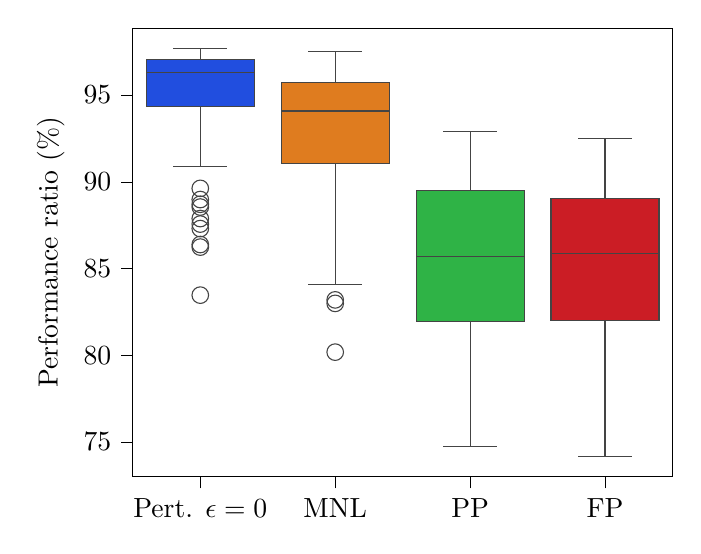
\begin{tikzpicture}

\definecolor{chocolate22312431}{RGB}{223,124,31}
\definecolor{darkgray176}{RGB}{176,176,176}
\definecolor{darkslategray68}{RGB}{68,68,68}
\definecolor{firebrick2032937}{RGB}{203,29,37}
\definecolor{limegreen4717970}{RGB}{47,179,70}
\definecolor{royalblue3378223}{RGB}{33,78,223}

\begin{axis}[
tick align=outside,
tick pos=left,
x grid style={darkgray176},
xmin=-0.5, xmax=3.5,
xtick style={color=black},
xtick={0,1,2,3},
xticklabels={Pert. \(\displaystyle \epsilon=0\),MNL,PP,FP},
y grid style={darkgray176},
ylabel={Performance ratio (\%)},
ymin=73.0126816492352, ymax=98.851891984976,
ytick style={color=black},
ytick={70,75,80,85,90,95,100},
yticklabels={
  \(\displaystyle {70}\),
  \(\displaystyle {75}\),
  \(\displaystyle {80}\),
  \(\displaystyle {85}\),
  \(\displaystyle {90}\),
  \(\displaystyle {95}\),
  \(\displaystyle {100}\)
}
]
\path [draw=darkslategray68, fill=royalblue3378223]
(axis cs:-0.4,94.3583668716296)
--(axis cs:0.4,94.3583668716296)
--(axis cs:0.4,97.0304994279352)
--(axis cs:-0.4,97.0304994279352)
--(axis cs:-0.4,94.3583668716296)
--cycle;
\addplot [darkslategray68]
table {%
0 94.3583668716296
0 90.8923771825346
};
\addplot [darkslategray68]
table {%
0 97.0304994279352
0 97.6773824242606
};
\addplot [darkslategray68]
table {%
-0.2 90.8923771825346
0.2 90.8923771825346
};
\addplot [darkslategray68]
table {%
-0.2 97.6773824242606
0.2 97.6773824242606
};
\addplot [black, mark=o, mark size=3, mark options={solid,fill opacity=0,draw=darkslategray68}, only marks]
table {%
0 87.8817328799838
0 87.5646932209679
0 89.6215083940763
0 87.3032659192475
0 88.5449661317598
0 86.2373659689477
0 86.3858890120452
0 83.4682240609051
0 88.7055814669542
0 88.9774803758999
};
\path [draw=darkslategray68, fill=chocolate22312431]
(axis cs:0.6,91.0542915481331)
--(axis cs:1.4,91.0542915481331)
--(axis cs:1.4,95.7218502384598)
--(axis cs:0.6,95.7218502384598)
--(axis cs:0.6,91.0542915481331)
--cycle;
\addplot [darkslategray68]
table {%
1 91.0542915481331
1 84.0683351615054
};
\addplot [darkslategray68]
table {%
1 95.7218502384598
1 97.5190151596301
};
\addplot [darkslategray68]
table {%
0.8 84.0683351615054
1.2 84.0683351615054
};
\addplot [darkslategray68]
table {%
0.8 97.5190151596301
1.2 97.5190151596301
};
\addplot [black, mark=o, mark size=3, mark options={solid,fill opacity=0,draw=darkslategray68}, only marks]
table {%
1 80.1832295616118
1 82.9924018720299
1 83.1940641618163
};
\path [draw=darkslategray68, fill=limegreen4717970]
(axis cs:1.6,81.9577093234914)
--(axis cs:2.4,81.9577093234914)
--(axis cs:2.4,89.493561829944)
--(axis cs:1.6,89.493561829944)
--(axis cs:1.6,81.9577093234914)
--cycle;
\addplot [darkslategray68]
table {%
2 81.9577093234914
2 74.7397800293973
};
\addplot [darkslategray68]
table {%
2 89.493561829944
2 92.900743210251
};
\addplot [darkslategray68]
table {%
1.8 74.7397800293973
2.2 74.7397800293973
};
\addplot [darkslategray68]
table {%
1.8 92.900743210251
2.2 92.900743210251
};
\path [draw=darkslategray68, fill=firebrick2032937]
(axis cs:2.6,81.9848971547146)
--(axis cs:3.4,81.9848971547146)
--(axis cs:3.4,89.0634049663873)
--(axis cs:2.6,89.0634049663873)
--(axis cs:2.6,81.9848971547146)
--cycle;
\addplot [darkslategray68]
table {%
3 81.9848971547146
3 74.1871912099507
};
\addplot [darkslategray68]
table {%
3 89.0634049663873
3 92.4757144002047
};
\addplot [darkslategray68]
table {%
2.8 74.1871912099507
3.2 74.1871912099507
};
\addplot [darkslategray68]
table {%
2.8 92.4757144002047
3.2 92.4757144002047
};
\addplot [darkslategray68]
table {%
-0.4 96.3142210188277
0.4 96.3142210188277
};
\addplot [darkslategray68]
table {%
0.6 94.0807111742749
1.4 94.0807111742749
};
\addplot [darkslategray68]
table {%
1.6 85.7174748323543
2.4 85.7174748323543
};
\addplot [darkslategray68]
table {%
2.6 85.8620096566213
3.4 85.8620096566213
};
\draw (axis cs:0,66.5528790652999) node[
  scale=0.75,
  anchor=base,
  text=black,
  rotate=0.0
]{\bfseries 95.17};
\draw (axis cs:1,66.5528790652999) node[
  scale=0.75,
  anchor=base,
  text=black,
  rotate=0.0
]{\bfseries 92.93};
\draw (axis cs:2,66.5528790652999) node[
  scale=0.75,
  anchor=base,
  text=black,
  rotate=0.0
]{\bfseries 85.56};
\draw (axis cs:3,66.5528790652999) node[
  scale=0.75,
  anchor=base,
  text=black,
  rotate=0.0
]{\bfseries 85.18};
\draw (axis cs:-1,66.8112711686574) node[
  scale=0.75,
  text=black,
  rotate=0.0
]{\bfseries \textbf{Average:}};
\end{axis}

\end{tikzpicture}
